%-------------------------------------------------------------------------------
% IPOL article about On Building an Accurate Stereo Matching System on Graphics Hardware article
% by Yohann Salaun & Pascal Monasse
% February 2013
%-------------------------------------------------------------------------------
\documentclass{ipol}

\ipolSetTitle{AD Census}
\ipolSetAuthors{Yohann Salaun$^1$ \& Pascal Monasse$^2$}
\ipolSetAffiliations{%
$^1$ Polytechnique, France (\texttt{yohann.salaun@polytechnique.org})\\
$^2$ Imagine, ENPC, France (\texttt{})}

\begin{document}

%-------------------------------------------------------------------------------
\begin{abstract}
This paper present a local stereo matching algorithm supposed to have good accuracy performances as shown by its position in Middlebury benchmark. Originally published in order to be developped on graphics hardware, only the accuracy performance will be studied in this article. The algorithm bases its matching cost with the AD-Census measure, aggregates in cross-based regions and finalizes it with scanline optimization. Methods are then used to detect outliers and correct them to finally give a disparity map that top performed in Middlebury benchmark.
\end{abstract} 

%-------------------------------------------------------------------------------
\section{Overview}

Stereo matching is one of the most active research areas in computer vision. Many algorithms have been proposed in the last decades and  \cite{stereoTaxonomy} presents and classify many of them.\\
Stereo algorithms can be split into 2 main families: \textbf{local} and \textbf{global} algorithm. The first one will only compare pixels from one picture to the other in order to find the best matches and compute the corresponding disparity map. The second one describes the disparity map computation problem as an energy minimization one and computes the disparity of each pixel at once.\\
Most of the time local methods are fast but lack of accuracy and global ones are accurate but take a lot of time to compute. The method \cite{adCensus}  presented below belongs to the local algorithm family and the aim of their author was to to produce an accurate real-time method with GPU parallelization. When the article was published (August 2011), this method was the top performer of Middleburry benchmark \cite{middleBench} and is now (January 2013) second top performer. The aim of this article is to study the quality of the disparity map produced by this algorithm, putting aside the GPU paralellization and the time performance.

%-------------------------------------------------------------------------------
\section{Matching cost computation}

\subsection{AD-Census}

The cost used in this algorithm is the combination of two other costs:\\
	- \textbf{ Absolute Difference} which computes the absolute difference of two pixel intensities.\\
	- \textbf{ Census} which computes the difference of two pixel local structures\\
\\ 
The absolute difference is a common matching cost, often used in disparity map computation for its good results. However it is lacking of accuracy in textureless regions. That is why the combination of two costs, supposed to improve the AD measure where its efficiency is too weak, has been used in this article.\\
The absolute difference cost is then given by the formula:
\[
	C_{AD}(p, pd) = \frac{1}{3} \sum_{i = R, G, B}  | I_i^{LEFT}(p) - I_i^{RIGHT}(p+d) | 
\]
Here and in the whole article, $p$ will be a pixel in the left picture and $p + d$ will be its correspondent with disparity $d$ in the right picture.\\
The census matching cost compares the local ordering of pixel intensities in a window of size 9 x 7.\\
The census cost formula can be given by:
\[
	C_{CENSUS}(p, pd) = \sum_{q \in windows(p)} I
\]
The combination of these two costs is made with the function $\rho$ defined by:
\[
	\rho(cost, \lambda) = 1 - e^{-\frac{cost}{\lambda}}
\]
This function allow a better combination of the two costs by mapping their values into [0;1] where 0 stands for a perfect match and 1 for a total mismatch. Moreover, it allows us to easily define the limit between inliers and outliers separately for each cost.\\

\subsection{ Cost aggregation }

Once the cost is initialized with AD-Census as explained above, it is aggregated, for a given disparity, in windows in order to increase matching accuracy. The method used is inspired by the one proposed by \textit{ Zhang et al.} \cite{costAggreg}.
The aggregation windows are computed independantly for each pixel and depends on the local structure of its neighbourhood (FIG. \ref{cost_computation}. The aim is to only take pixels that belong to the same structure in order to avoid occlusion issues.\\

\begin{figure}[h]
\begin{center}	
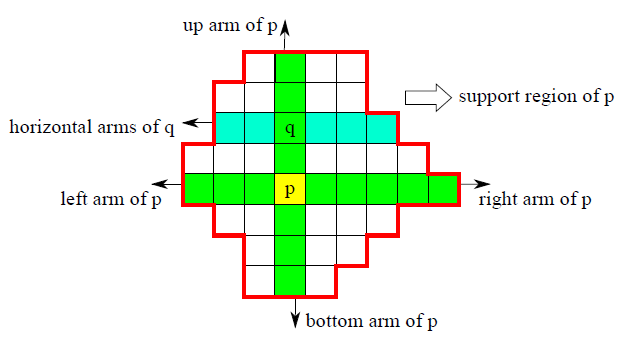
\includegraphics[scale=0.8]{Images/cost_computation.png}
	\label{cost_computation}
	\caption{ The adaptive windows only keeps pixel that have strong enough color similarities with the pixel in its center.}
\end{center}
\end{figure}

Thus, for each pixel $p$, upward, downard, leftward and rightward borders pixel $q$ are defined by being the last pixels in the given direction that assume:
\begin{equation}
	D_C(q, p) < \tau_1 \ \ and \ \ D_C(q, q_{predecessor}) < \tau_1
	\label{cost_agg1}
\end{equation}
\begin{equation}
	D_S(q, p) < L_1 
	\label{cost_agg2}
\end{equation}
\begin{equation}
	D_C(q, p) < \tau_2 < \tau_1 \ \ if \ \ L_2 <  D_S(q, p) < L_1
	\label{cost_agg3}
\end{equation}
where $D_C(p, q) = \max_{i \in R, G, B} |I_i(p) - I_i(q)|$ is the color distance between 2 pixels and  $D_S(p, q) = |p - q|$ is the spatial distance between 2 pixels.\\
Eq. \ref{cost_agg1} ensures that pixels which belong to the same window have a color similarity and that this similarity kept from the center of the window to the edge.\\
Eq. \ref{cost_agg2} defines a limit size for the window.\\
Eq. \ref{cost_agg3} allow bigger windows of size $L_1$ instead of $L_2$ only for textureless regions, when the pixels have strong color similarities.\\
Two adaptive windows can then be defined depending on the order of aggregation. For each pixel $p$, the cost is aggregated horizontally (resp. vertically) with the borders defined above and then the cost is aggregated once again vertically (resp. horizontally). See FIG. \ref{cost_aggregation}.\\
In order to get a stable cost volume, the cost is aggregated 4 times, twice horizontally first and twice vertically first.\\

\begin{figure}[h]
\begin{center}	
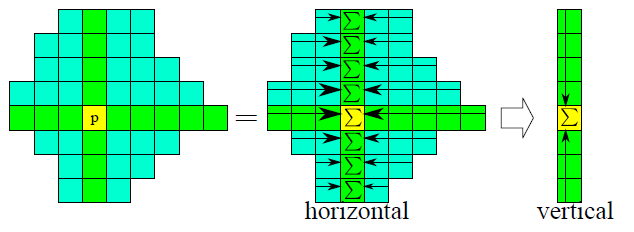
\includegraphics[scale=0.8]{Images/cost_aggregation.png}
	\label{cost_aggregation}
	\caption{ The aggregation is done one direction after the other with the corresponding border pixels.}
\end{center}
\end{figure}

For better matching results, a second aggregating step is then computed. It follows the multi-direction scanline optimizer developped by \textit{Hirschmuller REFFF}.\\
Four scanline optimizations are processed independantly, leftward, rightward, upward and downward. For a given direction $r$, the cost is updated from the first column/line to the last with the following formula:
\[
	C_r (p, d) =  C(p, d) + min( C_r(p, d) , C_r(p-r, d+1) + P_1, C_r(p-r, d-1) + P_1, \min_k C_r(p-r, k) + P_2) - \min_k C_r(p-r, k)	
\]
where $p-r$ is the previous pixel along the direction $r$.\\
$P_1 < P_2$ are parameters that penalize the disparity change between neighboring pixels. Thus, they depends on $D_1 = D_C(p, p-r)$ in the left picture and $D_2 = D_C(pd, pd-r)$ in the right picture. They are symmetrically set by the formula:
\[
	P_1 = \Pi_1, \ \ P_2 = \Pi_2, \ \ if \ \ D_1 < \tau_{SO} \ \ and \ \ D_2 < \tau_{SO}
\]
\[
	P_1 = \frac{\Pi_1}{4}, \ \ P_2 =\frac{\Pi_2}{4}, \ \ if \ \ D_1 > \tau_{SO} \ \ and \ \ D_2 < \tau_{SO}
\]
\[
	P_1 = \frac{\Pi_1}{4}, \ \ P_2 =\frac{\Pi_2}{4}, \ \ if \ \ D_1 < \tau_{SO} \ \ and \ \ D_2 > \tau_{SO}
\]
\[
	P_1 = \frac{\Pi_1}{10}, \ \ P_2 =\frac{\Pi_2}{10}, \ \ if \ \ D_1 > \tau_{SO} \ \ and \ \ D_2 > \tau_{SO} \\
\]
where $\Pi_1, \ \ \Pi_2 $ and $\tau_{SO}$ are parameters.\\
\\
Finally, the scanline optimization cost is the average of the 4 directionnal costs computed previously:
\[
	C(p, d) = \frac{1}{4} \sum_r C_r(p,d)
\]

---------------------------------------------------------------\\
There is no need for installation to use this class, just two files
need to be copied to the same directory were are the \LaTeX\ source
files. These files are the class itself, \verb|ipol.cls|, and the logo
file, that can be either \verb|ipol_logo.eps| if you compile with
\verb|latex| or \verb|ipol_logo.png| if you compile with
\verb|pdflatex|. If not sure, just copy the three of these files.

The minimal example of the class is as follows:
\begin{verbatim}
\documentclass{ipol}
\begin{document}
\end{document}
\end{verbatim}
It will only generates IPOL's header, including it's logo, and the
words ``title'' and ``authors'' where the title and authors should be
placed.  This example is useless but can be used to test your system.

This class is based on the standard 'article' class of \LaTeX\ and it
is used essentially in the same way. There are two main use
instruction: the layout must not be changed and title is not generated
with the usual \verb|\title|, \verb|\author|, \verb|\date|, and
\verb|\maketitle| commands. Let us discuss one by one.

This class was created to provide a uniform layout for IPOL articles,
so no command should be used that would change the page layout: do not
change paper size (it must be A4 paper), do not change the page
margins, do not change the font type, size, or color.

The commands \verb|\ipolSetTitle|, \verb|\ipolSetAuthors| and
\verb|\ipolSetAffiliations|, are provided by the IPOL class to set the
information needed to generate the title of the article. These
commands must be used in the preamble of the \LaTeX\ file, that is
between the \verb|\documentclass{ipol}| and \verb|\begin{document}|
commands. This is important, otherwise the title will not be generated
correctly. As the name of the commands imply, \verb|\ipolSetTitle| is
used to set the title of the article, \verb|\ipolSetAuthors| is used
to set the article's authors, and \verb|\ipolSetAffiliations| is used
to set the authors affiliations. This last command is optional. The
following is an example of how to use it:
\begin{verbatim}
\documentclass{ipol}
\ipolSetTitle{Ceci n'est pas un article}
\ipolSetAuthors{Rafael Grompone von Gioi}
\ipolSetAffiliations{CMLA, ENS Cachan, France}
\begin{document}
\end{document}
\end{verbatim}
If there are more than one author, and they have different affiliations,
they may be indicated as follows:
\begin{verbatim}
\documentclass{ipol}
\ipolSetTitle{Ceci n'est pas un article}
\ipolSetAuthors{Rafael Grompone von Gioi$^1$ \& Raphael Toucour$^2$}
\ipolSetAffiliations{$^1$ CMLA, ENS Cachan, France\\
                     $^2$ IIE, UdelaR, Uruguay}
\begin{document}
\end{document}
\end{verbatim}
For the rest, the class is used as the standard ``article'' class:
packages or definitions can be added in the preamble, and the main
text can contain sections, subsections, mathematics, figures, tables,
etc.

The rest of this document describes some special command for IPOL and
briefly comments on some conditions that will be imposed for a final
article, just before publishing at IPOL. (These restrictions are not
necessary for submissions but will reduce the work later.)

%-------------------------------------------------------------------------------
\section{Specific IPOL Commands}

Once an article is published at IPOL it will be assigned a DOI number
and a universal DOI web address to refer to it. The IPOL class
provides a command that will later contain the article's DOI number
(\verb|\ipolDOI|) and a command that will contain the article's web
address (\verb|\ipolLink|). These are the only reference that should
be used for the IPOL article itself and to its complementary contents
on the web.

These commands will have a default value in a preprint version, but
once the paper is accepted they will be replaced by the right value.
One may want to have a valid link while the article is being prepared
and peer reviewed. For that purpose, the command \verb|\ipolPreprintLink|
is used to set the article link \verb|\ipolLink| to a temporary
value. For example,
\begin{verbatim}
\ipolPreprintLink{https://tools.ipol.im/wiki/ref/manuscript_guidelines/}
\end{verbatim}
This command should be used in the document's preamble (i.e., after
\verb|\documentclass{ipol}| and before \verb|\begin{document}|).

The command \verb|\ipolLink| only provides the address of the
corresponding IPOL article. To produce a link with it or other
address, the command \verb|\href{}{}| should be used. The first
parameter is the link address while the second is the text that will
be shown in the resulting document. Also, to be able to read the
address in a printed version of the document, the address is also
printed as footnote. For example, the commands
\begin{verbatim}
\href{\ipolLink}{the article page}
\href{https://tools.ipol.im/wiki/ref/manuscript_guidelines/}{guidelines}
\end{verbatim}
produce the following links:
\href{\ipolLink}{the article page} and
\href{https://tools.ipol.im/wiki/ref/manuscript_guidelines/}{guidelines}.

Two particular environments are defined to generate two particular
parts of IPOL articles: \verb|ipolCode| and \verb|ipolSupp|. The first
one generates the ``Source Code'' description paragraph while the
second generates the ``Supplementary Material'' description
paragraph. These environment work similarly as the ``abstract'' and
should be used after the \verb|\begin{document}| and before the main
text of the article. The following is an example:
\begin{verbatim}
\documentclass{ipol}
\ipolSetTitle{Ceci n'est pas un article}
\ipolSetAuthors{Rafael Grompone von Gioi}
\begin{document}

\begin{abstract}
A short description of the article.
\end{abstract}

\begin{ipolCode}
Description of the source code to be found \href{\ipolLink}{here}.
\end{ipolCode}

\begin{ipolSupp}
Some articles could provide additional material, not part of the
peer reviewed article but related and useful. It should be found at
\href{\ipolLink}{the web page}.
\end{ipolSupp}

\section{Introduction}
The article main text starts here.

\end{document}
\end{verbatim}

%-------------------------------------------------------------------------------
\section{IPOL final article restrictions}

This document describes IPOL \LaTeX\ class that provides a uniform
layout for IPOL articles. Authors should also check the
\href{https://tools.ipol.im/wiki/ref/manuscript_guidelines/}{IPOL
  manuscript guidelines} where the requirements and suggestions about
the contents, style and description detail for IPOL articles are
described.

The PDF files for IPOL submissions are generated by the authors using
any method that produces a readable PDF file. Once an article is
accepted, however, the final version will be generated at IPOL servers
in order to provide PDF files with controlled sizes and resolutions
conditions. For that aim, there are some restrictions that must be
imposed to the source files. In what follows are described the main
restrictions, but more details are described
\href{https://tools.ipol.im/wiki/ref/manuscript_guidelines/}{here}.

The final documents will be generated using pdf\LaTeX. This forces
some restrictions, in particular the only graphical formats directly
accepted are PNG, JPEG and PDF itself. Images or figures in other kind
of formats should be converted to one of these.

The files and directories must follow a strict naming as defined
\href{https://tools.ipol.im/wiki/ref/manuscript_guidelines/}{here}.

Finally, the authors must warrant to be the authors of every part
of the final article, or must include permission of the copyright
holder. In particular, if images not owned by the authors are used,
the authors and permissions to be used must be included in the article.
For example, by adding a final section as follows:
\begin{verbatim}
\section*{Image Credits}

\includegraphics[height=2em]{image1.png}
\href{http://a.link.here}{Courtesy of Name Surname}
\\
\includegraphics[height=2em]{image2.png}
\copyright\ Pierre Dupont
\\
\includegraphics[height=2em]{image3.png}
the authors
\end{verbatim}

%-------------------------------------------------------------------------------
\section*{Image Credits}


\includegraphics[height=2em]{ipol_logo} \copyright\ IPOL (there's no
need to credit this image, here is used as an example.)

\section{References}

\begin{thebibliography}{9}
\bibitem{middleBench}
	D. Scharstein and R. Szeliski,
	\emph{ Middlebury benchmark}.
	vision.middlebury.edu/stereo/

\bibitem{adCensus}
	X. Mei, X. Sun, M. Zhou, S. Jiao, H. Wang, and X. Zhang,
	\emph{On building an accurate stereo matching system on graphics hardware}.
	GPUCV,
	2011.

\bibitem{stereoTaxonomy}
	D. Scharstein and R. Szeliski,
   	\emph{ A taxonomy and evaluation of dense two-frame stereo correspondence algorithms}.
	International Journal of Computer Vision, 
	47(1/2/3):7-42, 
	April-June 2002.

\bibitem{costAggreg}
	K. Zhang, J. Lu, and G. Lafruit,
	\emph{ Cross-based local stereo matching using orthogonal integral images}.
	 IEEE TCSVT,
	19(7):1073–1079,
	2009.

\end{thebibliography}

\end{document}
%-------------------------------------------------------------------------------
